\begin{figure}[!h]
\centering
\caption{Coefficient on population density $ \beta_t $ controlling for worker characteristics}
\subfloat[Cross-sectional gradient]{\includegraphics[width=.5\textwidth]{../2_analysis/output/figures/with_control_gradients_individual_l_czone_density_full_time}} \subfloat[Change in the gradient]{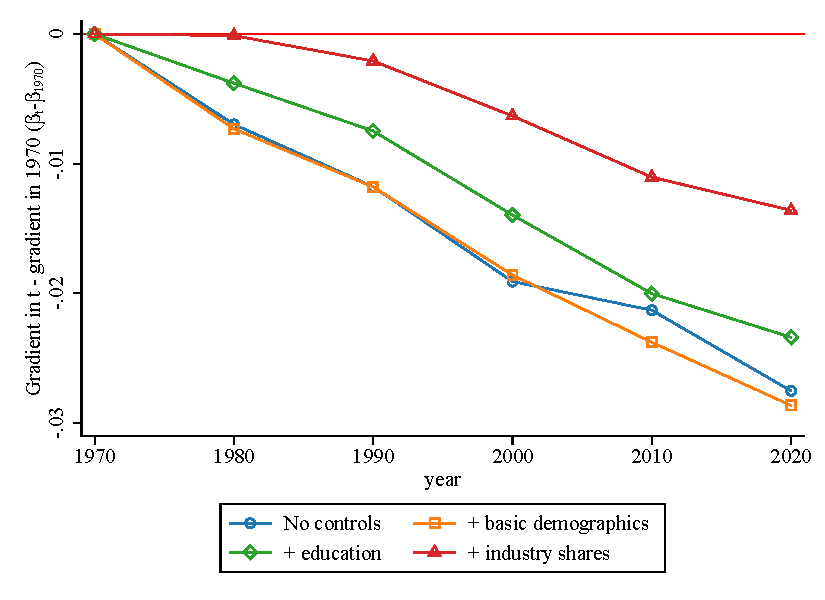
\includegraphics[width=.5\textwidth]{../2_analysis/output/figures/gradient_change_individual_l_czone_density_full_time}} \\ 
\par \begin{minipage}[h]{\textwidth}{\tiny\textbf{Note:} figure restricts to CZ with more than 1 people per km$^2$. The regressions are done on data aggregated at the CZ level. Basic individual level controls include full set of: race, age, marital status and foreign born dummies. Education is measured using a 4-level education dummies: HS dropout, HS graduate, some college and bachelor +. Bars show 95\% robust confidence intervals.}\end{minipage}
\end{figure}
